\chapter{Introducción}
\label{chap1}
\ifpdf
  \graphicspath{{Chapter1/Chapter1Figs/PNG/}{Chapter1/Chapter1Figs/PDF/}{Chapter1/Chapter1Figs/}}
\else
  \graphicspath{{Chapter1/Chapter1Figs/EPS/}{Chapter1/Chapter1Figs/}}
\fi

\markboth{\hfill \thechapter. Introducción}{\hfill \thechapter. Introducción}

El impacto ambiental que provocan los residuos sólidos municipales ha sido objeto de atención especial en las últimas décadas. La eliminación de los residuos sólidos urbanos es una preocupación creciente en todo el mundo, sin importar el tamaño ni las características socio-económicas de una ciudad. Muchas ciudades se han visto obligadas a evaluar su programa de gestión de residuos sólidos y examinar su relación costo-efectividad en términos de recolección, transporte, tratamiento y eliminación \citep{Karadimas2007OptimalAlgorithm}.

Según la literatura, en la Gestión de Residuos Sólidos (SWM, \textit{Solid Waste Management}) se estima que de la cantidad total de dinero gastado para la recogida, transporte y eliminación de residuos sólidos, aproximadamente el 60-80\% se gasta en la fase de Recolección de Residuos Sólidos (SWC, \textit{Solid Waste Collection}). Por lo general la SWC en los países en desarrollo se basa en la experiencia práctica y los métodos intuitivos, dando lugar a prácticas ineficientes y costosas, que afectan tanto a la salud pública como al medio ambiente. Por ende, incluso una pequeña mejora en la operación de recogida puede dar lugar a un ahorro importante en el costo total, motivo por el cual muchos municipios han realizado muchos esfuerzos en mejorar la gestión de la basura.

La Municipalidad de Asunción, de ahora en adelante MDA, cuenta con un conjunto de programas de trabajo anuales. En la Figura \ref{fig:porcentajePresupuesto}, se puede observar cómo la mayor parte del presupuesto total de la municipalidad correspondiente al año 2017, es destinado a los programas de acción. A su vez, dentro de estos programas, el que se lleva la mayor parte, y con una diferencia significativa sobre las demás, son los servicios de calidad en recolección y limpieza, como se muestra en la Figura \ref{fig:programaAccion}.

\begin{figure}[H]
    \centering
    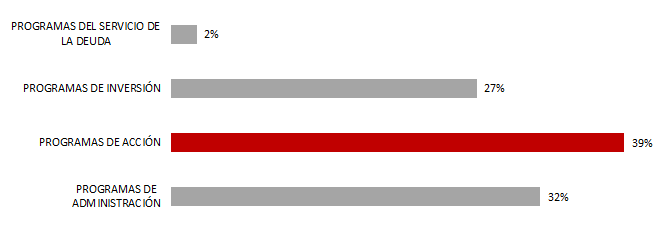
\includegraphics[width=14.5cm]{20181119_PresupuestoTotal2017.png}
    \caption{Representación porcentual del Presupuesto Total de la Municipalidad de Asunción discriminado por los programas para el año 2017. [Fuente: Portal de la Municipalidad de Asunción - Ejercicio Fiscal 2017]}
    \label{fig:porcentajePresupuesto}
\end{figure}

\begin{figure}[H]
    \centering
    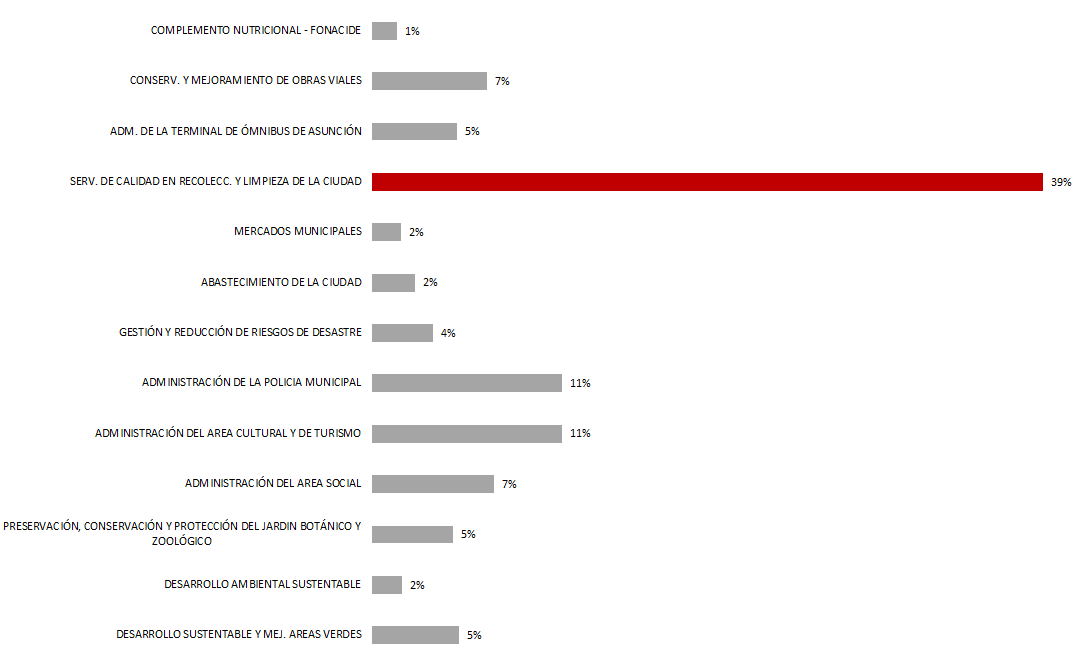
\includegraphics[width=15cm]{20181119_PresupuestoAccion2017.png}
    \caption{ Representación porcentual del Presupuesto correspondiente a los subprogramas del Programa de Acción correspondientes al año 2017. [Fuente: Portal de la Municipalidad de Asunción - Ejercicio Fiscal 2017]}
    \label{fig:programaAccion}
\end{figure}

\section{Antecedentes}

Cuando se habla de la problemática de la gestión de residuos sólidos, es sabido que existen numerosos estudios y trabajos científicos que se han realizado al respecto con el propósito de resolverla usando objetivos económicos y/o ambientales como criterios para la toma de decisiones. Hasta hoy día se estudian distintas técnicas que puedan permitir mejorar el proceso, como mencionan  \citet{Tchobanoglous1993IntegratedIssues}, no existe un conjunto universal de reglas que puedan aplicarse a todas las situaciones.

% En \citet{VitorinodeSouzaMelare2017TechnologiesReview} se realiza una revisión de los diversos procesos relacionados a la gestión de residuos sólidos y los agrupa en seis categorías: la gestión de recogida, recorrido y transporte; gestión y seguimiento de contenedores; reciclaje de residuos sólidos y gestión de residuos electrónicos; administración pública y desarrollo sostenible; métodos de previsión y planificación; y determinación de sitios de disposición de residuos.

% VRP CVRP VRPTW
La SWC muchas veces se trata como un Problema de Enrutamiento de Vehículo (VRP, \textit{Vehicle Routing Problem}) o su variación, un Problema de Enrutamiento de Vehículo Capacitado(CVRP, \textit{Capacitated Vehicle Routing Problem}). \citet{Akhtar2017BacktrackingOptimization} resuelven el CVRP utilizando el algoritmo  meta-heurístico de búsqueda hacia atrás (BSA, \textit{Backtracking Search Algorithm}), mientras que \citet{Mohammed2017SolvingSolution} utilizan un algoritmo genético (GA, \textit{Genetic Algorithm}). También se afrontaron trabajos como un Problema de Erutamiento de Vehículos con Ventana de Tiempo (VRPTW, \textit{Vehicle Routing Problem with Time Window}), como en \citet{Ombuki-Berman2007WASTEALGORITHMS}, donde se ha resuelto utilizando un GA multi-objectivo.

% TSP
Otros trabajos de la literatura tratan como un Problema del Vendedor Viajante (TSP, \textit{Travelling Sales Problem}). En \citet{Billa2014GISOptimization} el enrutamiento óptimo se desarrolla un método basado en el TSP y luego se integra con ArcInfo GIS utilizando programación lineal(LP, \textit{Linear Programming}). \citet{Karadimas2007OptimalAlgorithm} implementan un sistema de colonia de hormigas (ACS, \textit{Ant Colony System}), el cual fue modelado como un TSP asimétrico (ATSP, \textit{Asymmetric TSP})

% PCC y DRPP rural abierto CARP
\citet{Vecchi2016ACollection} presentan un modelo formulado como un problema de programación lineal de enteros mixtos (MILP, \textit{Mixed Integer Linear Programming}) para resolver el Problema de Enrutamiento de Arco Capacitado (CARP \textit{Capacitated Arc Routing Problem}). Por otro lado, \citet{Braier2017AnArgentina}, resolvieron mediante un modelo de programación entera un caso particular del problema del cartero rural abierto dirigido (RPP, \textit{Rural Postman Problem})

%  \cite{Petrik2016OPTIMIZATIONPAIRING} utilizan Teoría de Grafos junto con el método de emparejamiento mínimo para optimizar la ruta de recolección.

La herramienta ArcGIS Network Analytics (NA) es utilizada ampliamente en la búsqueda por minimizar la distancia y el tiempo de las rutas actuales de los camiones recolectores de residuos sólidos \citep{Kallel2016UsingTunisia, Malakahmad2014SolidMalaysia}. Existen además implementaciones comerciales similares a la solución ha proponer, entre ellas se encuentran \textit{MapInfo Software}, \textit{RouteSmart}, \textit{Waste Route Software}, \textit{RouteViewPro}.
% Agregar las implementacion libres.

En este trabajo se propone el desarrollo de una herramienta, denominada de ahora en más \textit{TapeYty}, que optimice el camino seguido por los vehículos de recolección de basura de la ciudad de Asunción mediante técnicas de programación matemáticas, y consecuentemente, genere beneficios principalmente en los aspectos económicos y ambientales.

\section{Justificación}
 Actualmente, los choferes de los vehículos recolectores de basura de la ciudad de Asunción trazan los caminos a seguir en base a su experiencia, es por ello que se ha visualizado la necesidad de optimizar el recorrido realizado para la recolección de residuos, reduciendo el costo y el tiempo de cada recorrido. A su vez, permitirá a la MDA gestionar de manera eficiente dichos recorridos a través de una aplicación, que permitirá actualizar el estado de las calles de la ciudad, es decir, si esta puede o no ser transitada por el vehículo recolector. La MDA podrá contar con una aplicación que garantice que todos los ciudadanos reciban el servicio de recolección domiciliaria.

El ingreso promedio de personas en ómnibus del transporte público y vehículos privados de los municipios aledaños, es alrededor de 1.320.000 a diario \citep{DiarioABCColor2016PorColor}, es así que no sólo los ciudadanos que residen en la ciudad de Asunción serán beneficiados con un servicio más eficiente, sino las miles de personas, que ingresan diariamente a la ciudad, ya que al reducir el tiempo del vehículo recolector en tránsito se reduce el tráfico generado por los mismos y los problemas de contaminación por los líquidos y gases que dejan a su paso.

Este proceso permitirá al personal encargado de la recolección de residuos agilizar su trabajo ya que pasarán menos tiempo en el vehículo recolector, mejorando así su calidad de vida.
 
Por todo lo expuesto, se considera plenamente justificada la investigación y propuesta de solución de este trabajo de fin de carrera, pues nos permitirá como ciudadanos retribuir en parte al Estado los beneficios y conocimientos que hemos adquirido a través de nuestra carrera en la Universidad.

\section{Objetivo General}
El objetivo general de este trabajo de investigación es el de proponer una solución que optimice el recorrido de los vehículos de recolección de basura domiciliaria de la Dirección Servicios Urbanos (DSU) de la MDA.

\section{Objetivos Específicos}

Los objetivos específicos que se han trazado en este trabajo son los siguientes:

\begin{enumerate}
    \item \textbf{Investigar} sobre técnicas de optimización para obtener el camino óptimo. 
    \item \textbf{Identificar} los factores que influyen en la recolección domiciliaria de la DSU.
    \item \textbf{Aplicar un modelo matemático} de optimización que mejor se ajuste a las reglas de negocio del caso de estudio.
    \item \textbf{Proponer y desarrollar un prototipo de aplicación GIS} que permita configurar los parámetros de entrada del problema y despliegue la ruta óptima para cada zona de recolección.
    \item \textbf{Comparar} resultados de la aplicación desarrollada con los recorridos que actualmente son realizados, y de esta manera validar los resultados obtenidos.
\end{enumerate}


\section{Organización del Trabajo}

La organización del presente trabajo se completa de la siguiente manera:

\begin{itemize}
    \item En el \textbf{capítulo 2} se presentan los conceptos básicos que describen la gestión de residuos sólidos municipales y el caso de estudio, la ciudad de Asunción.
    \item En el \textbf{capítulo 3} se presentan conceptos básicos sobre Sistemas de Información Geográfica y bases de datos espaciales.
    \item En el \textbf{capítulo 4} se presentan las distintas técnicas de optimización.    
    \item En el \textbf{capítulo 5} se plantea de manera formal el problema que se intenta resolver. Se explican las formulaciones utilizadas, así como una explicación detallada de la implementación de la herramienta \textit{TapeYty}. 
    \item En el \textbf{capítulo 6} se visualizan y se discuten los resultados de la propuesta.
    \item En el \textbf{capítulo 7}, se finaliza el trabajo de investigación presentando las conclusiones generales, así como los aportes, aprendizajes y trabajos futuros continuando esta línea de investigación.
    % \item En el \textbf{capítulo ANEXOS}
\end{itemize}